\documentclass[a4paper,utf8]{article}
\usepackage[heading,fancyhdr]{ctex}
\usepackage{amsmath,amssymb,geometry,lastpage,ulem}
\usepackage{array,tabularx,siunitx,graphicx}
\geometry{
    top=25.4mm, 
    left=30mm, 
    right=30mm, 
    bottom=35mm,
    headsep=5.9mm,
}
\pagestyle{fancy}
\ctexset{
    section = {format+=\raggedright}
}
\newcommand{\fgref}[1]{图~\ref{#1} }
\newcommand{\seqref}[1]{式~(\ref{#1})}
\newcommand{\qrange}[3]{\qtyrange[range-phrase = \text{$\sim$},range-units =single]{#1}{#2}{#3}}
\fancyhf{} \fancyhead[C]{材料科学基础实验} \fancyfoot[C]{\thepage~/~\pageref{LastPage}}
\begin{document}
\begin{center}
    {\mbox{}\\[7em]\zihao{2}\bfseries\songti%
    材料科学基础实验报告}\\[34mm]
    {\zihao{-3}\bfseries\songti
    实验名称:\uline{\hfill\mbox{四探针法测量半导体电阻率和薄层电阻}\hfill} \\[2.9mm]
    学\quad 号:\uline{\makebox[25mm]{22301077}}\hfill
    姓\quad 名:\uline{\makebox[25mm]{张蕴东}}\hfill
    班\quad 级:\uline{\makebox[25mm]{22高分子}} \\[2.9mm]
    合作者:\uline{\makebox[25mm]{无}}\enspace~
    桌\quad号:\uline{\makebox[25mm]{}}\hfill\mbox{}\\[2.9mm]
    指导教师:\uline{\makebox[30mm]{艾斌}}\hfill\mbox{} \\[2.9mm]
    实验日期:\uline{\makebox[30mm]{2024.3.8}}\hfill\mbox{} \\[58.7mm]
    } 
    {\zihao{4}\bfseries\songti
    实验考核\\[3mm]
    \extrarowheight=3mm
    \begin{tabularx}{150mm}{|X|X|X|X|X|}\hline
        \hfil 项目 \hfil  & \hfil 实验预习 \hfil & \hfil 实验过程 \hfil & \hfil 分析与讨论 \hfil & \hfil 总评 \hfil \\[3mm] \hline
        \hfil 评价 \hfil &  &  &  &  \\[3mm] \hline
    \end{tabularx}
    }
\end{center}\newpage
\section{实验目的}
    \begin{itemize}
        \item 理解四探针方法测量半导体电阻率和薄层电阻的原理;
        \item 学会用四探针方法测量半导体电阻率和薄层电阻;
        \item 针对不同几何尺寸的样品,了解其修正方法;
        \item 了解影响测量结果准确性的因素及避免方法
    \end{itemize}
\section{实验原理}%简单描述,含必要的公式和附图;
    \subsection{半导体材料体电阻率的测量}
        \subsubsection{半无穷大样品体电阻率的测量}
            在电阻率分布均匀的半无穷大样品表面上,若电流 I 通过探针以点电流源的形式注入到半导体材料内部,则电流密度在材料内部是均匀分布的,具体是以探针尖为球心沿径向放射状分布。四探针法测量半导体材料体电阻率采用四根金属探针排成一列,并且四根金属探针的间距相等,均为 $S$。将四根金属探针压在一块半无穷大的半导体材料表面上,当 1、4 探针通以电流 $I$(探针 1 为正极,探针 4 为负极),2、3 探针上测得的电压为 $V_{23}$ 时,只要样品厚度及边缘与探针的最近距离大于四倍探针间距,半无穷大样品的体电阻率 $\rho$ 可表示为:
            \begin{equation}
                \rho = 2\pi S\cdot\frac{V_{23}}{I} \label{eq:0}
            \end{equation} 
            半导体材料的电阻率对温度比较灵敏,因此,测试半导体材料的电阻率时不但要记录测试的环境温度,还要将该温度下的实测电阻率修正到 23℃下的电阻率,引入修正系数 $F_T$ : 
            \begin{equation}
                \rho =\frac{2\pi S}{F_T}\cdot\frac{V_{23}}{I}
            \end{equation}
        \subsubsection{无穷大薄样品体电阻率的测量}
            类似前面的分析,无穷大薄样品的体电阻率 $\rho$ 可表示为:
            \begin{equation}
                \rho =\frac{\pi V_{23}}{I \ln 2} \label{eq:1}
            \end{equation}
    \subsection{半导体材料电阻的测量}        
        \subsubsection{半导体薄层电阻(或方块电阻)的测量}
            如果扩散片的结深用 $X_j$ 表示,根据定义,方块电阻 $R_{sq}$ 可表示为:
            \begin{equation}
                R_{sq}=\rho\frac{L}{L\cdot X_{j}}=\frac{\rho}{X_{j}} \label{eq:2}
            \end{equation}
            将 \seqref{eq:1} 代入 \seqref{eq:2} 得:
            \begin{equation}
                R_{sq}=4.5324\frac{V_{23} d}{I} \label{eq:3}
            \end{equation}
            实际测量中,只要薄层的厚度小于 $0.5S$,并且样品面积相对于探针间距 $S$ 可视为无穷大时,就可以利用\seqref{eq:3}计算薄层电阻。如果不能将样品的横向面积视为无穷大,也需要使用包含修正因子 $F$ 的公式来计算方块电阻:
            \begin{equation}
                R_{sq}= F \frac{V_{23}}{I} \label{eq:4}
            \end{equation}
        
\section{实验仪器}%规格及参数
    KDY-1 型四探针电阻率/方阻测试仪,一台计算机;p 型单晶硅棒(电阻率样品)、p 型单晶硅片(薄样品)、p 型硅基底上的 n 型扩散片(薄层电阻样品)各一个
\section{实验过程}%简述主要过程和实验内容
    \subsection{测量样品电阻率或方块电阻的操作步骤}
    \begin{enumerate}
        \item{.} 打开 KDB-1 四探针测试仪后面板上的电源开关,此时恒流源已开启,测试电流自动处于 \SI{1}{\milli\ampere} 档。根据测试目的,将测试仪后面板上的 “电阻率/方块电阻测试切换开关”( $\rho/R$ 开关)拨到相应位置。
        \item{.} 将样品置于样品台上,旋转测试架上的手轮使探针下降,同时调整样品位置,使四根探针正好落在样品的测试点。当探针快要接触样品时,应缓慢旋转手轮,使探针缓慢轻压在样品上。当听到主机传来“咔嗒”一声、且前面板左侧的两块绿字电表有数值显示,即表示探针与样品已接触到位,应立即停止旋转手轮。
        \item{.} 根据附表给出的推荐值,并通过选择合适的测试电流档位和恒流源电压档位,调节测试电流和恒流源电压旋钮,使测试电流达到合适的值,此时,电压表显示的 V23 应出现尽可能多的有效数字,且电压值在测试电流不变的前提下能长时间保持稳定,而且正测和反测得到的 V23 的绝对值差别也不大。
        \item{.} 记录此时的测试电流 I 和电压 V23 的值,由相应公式计算样品的电阻率或方块电阻。测量完毕,升起探针,取走样品。
    \end{enumerate}
    \subsection{测量 p 型硅棒的电阻率}
        使用厂家推荐的测试电流对硅棒横截面上五个不同位置处(中心点和距离圆心 1/3 半径处的 4 个等距点)的电阻率进行测量。为了减小测量误差,对同一点的测量分别进行正向和反向测量。将实验结果记录到表中,使用 \seqref{eq:0} 计算电阻率 $\rho (T)$。利用附录将测得的电阻率修正到 \SI{23}{\degreeCelsius}。此外,利用下面的公式计算电阻率分布的不均匀度。
    \subsection{测量 p 型单晶硅片(薄样品)的电阻率}
        \begin{enumerate}
            \item 直读法,根据样品厚度和附表 4 得到直读电流的值,并将其设置为测试电流,直接
            从电压表上读取样品的电阻率。
            \item 选择合适的测试电流 I 和测得的电压 $V_{23}$,采用 $\rho(T)=\frac{V_{23}}l\cdot d\cdot F_{SP}\cdot F(d/S)\cdot F(S/D)$ 计算硅片的电阻率。对硅片中心位置处的电阻率测量 5 次。每次测量完毕后,升起探针,将硅片逆时针旋转 $\SI{30}{\degree} \sim  \SI{35}{\degree}$ 进行下一次测量。同一位置正向和反向各测量一次,并将测量结果修正到 \SI{23}{\degreeCelsius}。
        \end{enumerate}
    \subsection{测量 p 型单晶硅衬底上的 n 型扩散片的方块电阻 }
        扩散片的结深 $X_j$ 和尺寸由老师现场提供。由于待测扩散片近似正方形,故取最短的边长作为扩散片的直径 $D$ 。将探针压在扩散片的中心位置进行方块电阻的测量。
        \begin{enumerate}
            \item 直读法,设置合适的测试电流,从电压表上直接读出样品的方块电阻。
            \item 根据测试电流、电压 $V_{23}$ 以及扩散片的尺寸,利用\seqref{eq:4}计算扩散片的方块电阻。需要测量两个位置的方块电阻,即在第一次测量完成之后将样品旋转 \SI{90}{\degree} 再测量一次。同一位置正向和反向各测量一次。
        \end{enumerate}
    \subsection{测量两种透明导电玻璃的方块电阻}
        本实验提供两种透明导电玻璃(FTO 导电玻璃和 ITO 玻璃),测试方法及要求与测试扩散片一致。

\section{实验数据与结果}
    表格随附
\section{不确定度分析}
    不确定度主要来源为恒流源,数字电压表与硅片厚度测量结果。已知数字电压表的测试量程为 \qrange{0.2}{50}{\mV},分辨率优于 $ \pm 0.05 \% $ 。在 $ 1 \unit{\mA} $ 电流档,恒流源最大允许误差为$\pm 0.02 \unit{\mA}$;在 $ 10 \unit{\mA} $ 电流档,恒流源最大允许误差为 $ \pm 0.1 \unit{\mA} $ 。硅片厚度测量结果的相对不确定为 $ \pm 0.2\% $。探针间距修正因子 $ F_{sp}$、样品厚度修正因子 $ F(d/S) $和直径修正因子 $ F(S/D) $ 引入的不确定度可以忽略。假定矩形分布来评估仪器精度引入的不确定度。\par
    材料各处存在一定的性能差异,认可其不同位置的测量结果存在变化的合理性,此处计算B类不确定度,可以得到下表:\par
    \begin{table}[!ht]
        \centering\begin{tabular}{c c c}\hline
            直接测量量 & 精度 & B类不确定度 \\ \hline
            \makebox[50mm]{数字电压表} & $\pm 0.025 \unit{\mV}$ &\makebox[50mm]{0.015} \\
            恒流源( $ 1 \unit{\mA} $ 档) & $ \pm 0.02 \unit{\mA}$ & 0.012 \\
            恒流源( $ 10 \unit{\mA} $ 档) & $ \pm 0.1 \unit{\mV}$ & 0.058 \\
            硅片厚度 &  & 0.2\% \\\hline
        \end{tabular}
    \end{table}
    本次误差传递时采用 Wolfram Mathematica 语言编写的程序进行自动处理。介绍编程语言并非本实验的目的,源代码如下,EP 为合成不确定度,EPF 为误差传递方程:
    \newpage
    \begin{figure}[!ht]\centering
        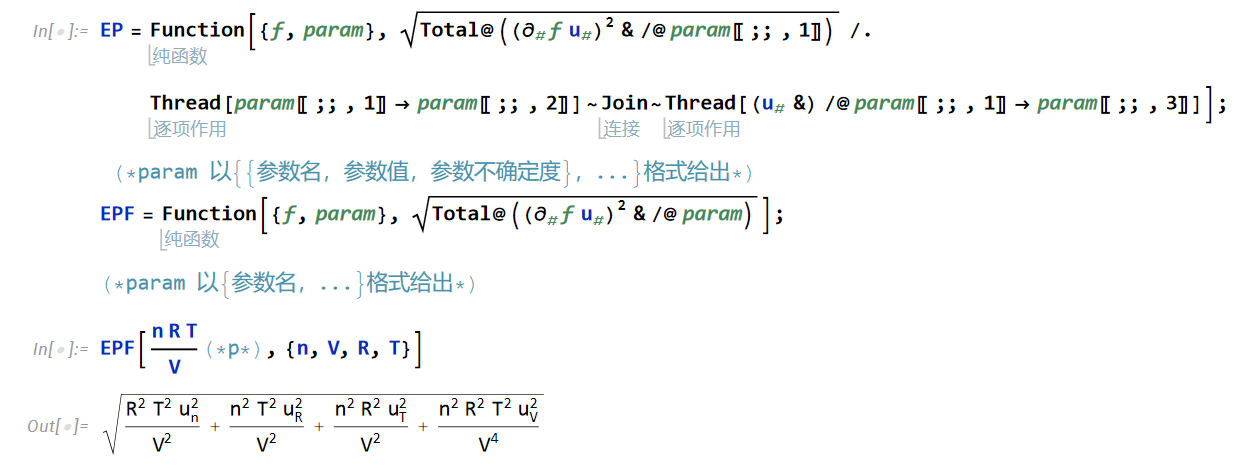
\includegraphics[width=150mm]{EF.png}
    \end{figure}
    \subsection{测量 p 型单晶硅片(薄样品)的电阻率}
        由于每次测量的方向不同,电流不同,故对测量 1 进行分析,过程如下:\par
        \begin{figure}[!ht]\centering
            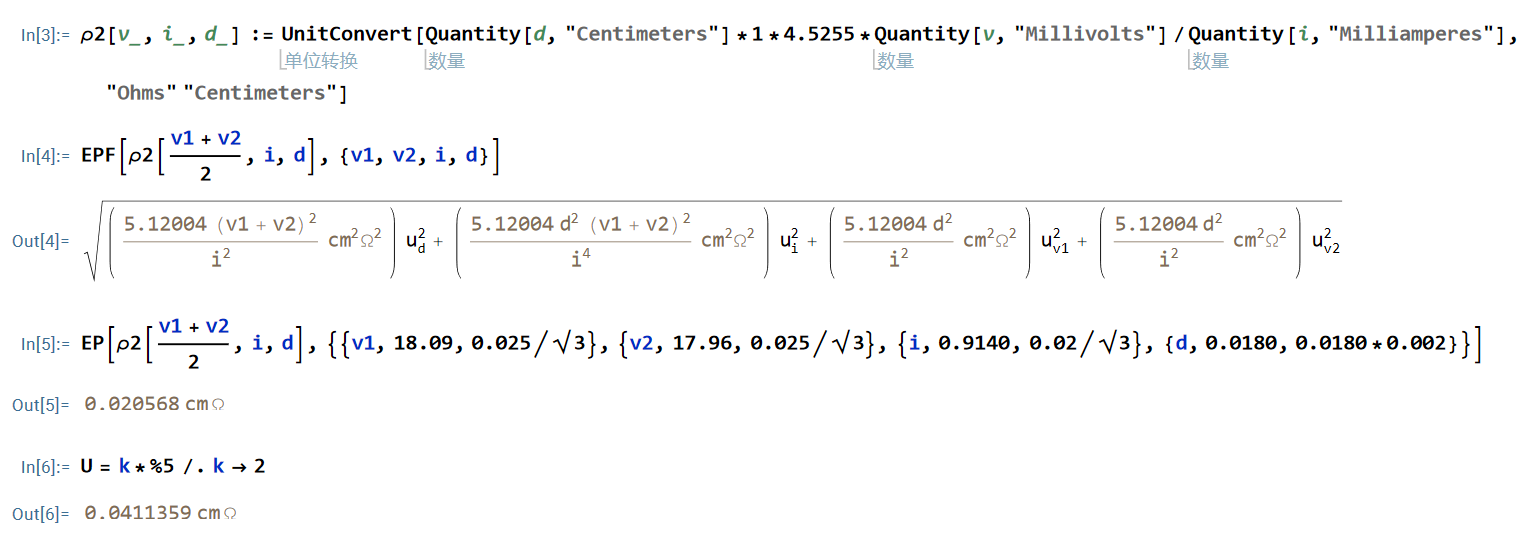
\includegraphics[width=150mm]{result.png}
        \end{figure}
        最后得到的拓展不确定度为:
        \begin{equation*}
            \rho_T = ( 1.606 \pm 0.042 ) \unit{\ohm\cm}
        \end{equation*}
        其中在“$\pm$”号后的数为扩展不确定度 $U=ku_c$ 的数值, $ U $ 是由 $ u_c= 0.020568 \unit{\ohm\cm}$ 和 $ k = 2 $ 确定的, $k$ 是基于矩形分布得到的,自由度在讲义中未提到。确定区间的包含概率在讲义中未提到。\par
        关于其他的实验的误差分析,讲义未提出要求,但值得注意的是:
        \begin{enumerate}
            \item 对于测量 p 型硅棒的电阻,由于其测试的位置在发生改变,即使测试电流相同,处理时不应计算 A 类不确定度,否则电阻率不均匀度将不存在物理意义,仅仅反映测量的不准确性。故实际误差分析的过程与测量 p 型单晶硅片(薄样品)的电阻率相比,无需考虑 d 的影响。
            \item 对于测量 p 型单晶硅衬底上的 n 型扩散片的方块电阻,若扩散片的方块电阻不会随着样品转角而发生变化,在不同的测试电流下,应当用统计方法处理。校准设计方案的应用是一个很好的例子,通常用最小二乘法评定未知值的实物量具(如量块和标准砝码)与已知值的参考标准比较结果的短期和长期随机变化引入的不确定度。在这种相对简单的测量情形下,不确定度分量通常通过数据的统计分析来评定,这些数据是在一套测量程序中将与其有关的量设计许多不同值来获得,这就是所谓的方差分析。
            \item 对于测量两种透明导电玻璃的方块电阻,则可以参考测量 p 型单晶硅衬底上的 n 型扩散片的方块电阻所用的最小二乘法通过数据的统计分析来评定不确定度。
        \end{enumerate}
        综上所述:如果重新进行该实验测量,我可以通过以下方法来提高不确定度的精度:
        \begin{enumerate}
            \item 对于测量 p 型硅棒的电阻,在每一个位置都正测反测多组,计算合成不确定度时就可以加入 A类不确定度项。若要计算电阻率不均匀度的不确定度,一样可以使用误差传递公式来计算。
            \item 对于测量 p 型单晶硅衬底上的 n 型扩散片的方块电阻,假定扩散片的方块电阻不会随着样品转角而发生变化,在每一个样品转角也都进行数次正测反测,最后利用多次的结果计算最小二乘法拟合直线。拟合直线的斜率和方差作为电阻率合成不确定度的分量(详见 GB/T27418—2017 中 F.3.4章节)
            \item 对于测量两种透明导电玻璃的方块电阻,则可以参考测量 p 型单晶硅衬底上的 n 型扩散片的方块电阻所用的最小二乘法通过数据的统计分析来评定不确定度,每一个样品转角也都进行数次正测反测,最后利用多次的结果计算最小二乘法拟合直线 $\dotsc$
        \end{enumerate}
\section{结果分析与讨论}
    从测量 p 型硅棒的电阻率实验数据可以看出,考虑测量误差的情况下,硅棒横截面上五个位置处的电阻率仍然有3\%以上的不均匀度,暗示我们不应该把这些不均匀简单当成是测量的随机波动,应当更进一步去思考其存在的内涵。不均匀可以来自原子的周期排布对电子波函数的调制;可以来自材料中的杂质和缺陷,这些杂质和缺陷会散射电子,改变电子的运动方向,不改变电子的速度;即使一个杂质都没有,在任何有限温度下,晶格都会在平衡位置左右震动。这种震动也散射电子,并且既改变电子的运动方向,也改变电子的运动速度。这种散射也带来电阻。由于晶格的震动强度与温度相关,所以这种散射也强烈地依赖温度。在低温下,晶格震动带来的电阻会变得很小。此外,在测量 p 型单晶硅衬底上的 n 型扩散片的方块电阻实验中,异质结的光生伏特作用对于测量也有一定的干扰。总结起来,本次实验可以通过控制好温度、避光、屏蔽外在电磁信号来减小误差,但材料本身性质引起的测量结果不同是不可以消除的,反而是值得去关注的重点。
\section{思考题} 
    \subsection{电阻率和方块电阻的测量结果的误差来源有哪些?应如何避免?}
        \begin{enumerate}
            \item 仪器的测量精度导致的误差 $\rightarrow $ 多次测量取平均值
            \item 测量条件的不完全一致导致的误差 $\rightarrow $ 尽可能保证在相同环境下进行实验
        \end{enumerate}
    \subsection{影响测量结果准确性的外界因素有哪些?应如何避免?}
        \begin{enumerate}
            \item 温度 $\rightarrow $ 晶格的震动强度与温度相关,因此半导体材料的电阻率对温度敏感,所以应该恒温下进行测试
            \item 污渍 $\rightarrow $ 由于样品的重复使用,样品上的灰尘和油污也会影响测试结果,可以先用酒精清洗再测试
        \end{enumerate}
\end{document}